\section{Anàlisis i preprocessat de dades}

\subsection{Preprocessat inicial}
Una vegada importem el dataset, es pot veure que hi ha bastantes cel·les buides i altres amb el string \texttt{`NaNN'}. Per solucionar aquesta inconsistència, s'han reemplaçat tots aquests valors per \texttt{pd.NA}.

Per altra banda, s'ha declarat el tipus de cada variable correctament (com a numèriques o com a categòriques) seguint la informació que es proporciona en el metadata file (que es pot trobar en \cite{misc_cirrhosis_patient_survival_prediction_878}).

A més, com que la variable ID no és res més que l'identificador dels pacients, i no serà necessari pel nostre estudi, s'ha decidit eliminar del dataset per no haver d'eliminar-la manualment a cada procés. És a dir, entrenar un model de predicció tenint en compte l'ID del pacient no té cap sentit i només pot portar a overfitting (si troba patrons entre la variable objectiu i la variable ID). A més, a l'hora de fer gràfics no és una variable que aporti cap informació, ja que és categòrica i amb tantes classes úniques com files hi ha al dataset, de manera no es podrien interpretar els plots de cap manera.

Addicionalment, per una millor comprensió de certes variables, s'ha decidit reanomenar els seus valors, tenint en compte el metadata file, de la següent manera:
\begin{itemize}
	\item \textbf{Variable Status:}
	\begin{itemize}
		\item \textbf{`C'} $\rightarrow$ `Alive'.
		\item \textbf{`CL'} $\rightarrow$ `Liver Transplant'.
		\item \textbf{`D'} $\rightarrow$ `Dead'.
	\end{itemize}
	
	\item \textbf{Variable Edema:}
	\begin{itemize}
		\item \textbf{`N'} $\rightarrow$ `NoEdema'.
		\item \textbf{`S'} $\rightarrow$ `EdemaResolved'.
		\item \textbf{`Y'} $\rightarrow$ `EdemaPersistent'.
	\end{itemize}
	
	\item \textbf{Variable Drug:}
	\begin{itemize}
		\item \textbf{`D-penicillamine'} $\rightarrow$ 1.
		\item \textbf{`Placebo'} $\rightarrow$ 0.
	\end{itemize}
	
	\item \textbf{Variables Ascites, Hepatomegaly i Spiders:}
	\begin{itemize}
		\item \textbf{`Y'} $\rightarrow$ 1.
		\item \textbf{`N'} $\rightarrow$ 0.
	\end{itemize}	
\end{itemize}

Una vegada realitzats aquests canvis, es pot començar a treballar amb el dataset correctament.

\subsection{Anàlisis estadístic de les variables}
El primer que s'ha fet per entendre el dataset i poder treballar amb ell és realitzar un anàlisis estadístic de cada una de les variables que el formen. A més, per les variables numèriques podem analitzar la distribució que segueixen mitjançant un histograma, mentre que per les categòriques podem realitzar countplots per veure la distribució entre les seves classes i com de balancejades estan.

\subsubsection{Variables numèriques}
En les taules \ref{tab:num-stats-1} i \ref{tab:num-stats-2} es poden veure estadístiques sobre totes les variables numèriques del dataset (obtingudes mitjançant la comanda \texttt{data.describe()} de la llibreria \texttt{pandas}).

% Table 1
\begin{table}[H]
\centering
\begin{tabular}{lrrrrrr}
\hline
\textbf{Statistic} & \textbf{N\_Days} & \textbf{Age} & \textbf{Bilirubin} & \textbf{Cholesterol} & \textbf{Albumin} & \textbf{Copper} \\ 
\hline
count & 418.0 & 418.0 & 418.000000 & 284.0 & 418.000000 & 310.0 \\ 
mean & 1917.782297 & 18533.351675 & 3.220813 & 369.510563 & 3.497440 & 97.648387 \\ 
std & 1104.672992 & 3815.845055 & 4.407506 & 231.944545 & 0.424972 & 85.61392 \\ 
min & 41.0 & 9598.0 & 0.300000 & 120.0 & 1.960000 & 4.0 \\ 
25\% & 1092.75 & 15644.5 & 0.800000 & 249.5 & 3.242500 & 41.25 \\ 
50\% & 1730.0 & 18628.0 & 1.400000 & 309.5 & 3.530000 & 73.0 \\ 
75\% & 2613.5 & 21272.5 & 3.400000 & 400.0 & 3.770000 & 123.0 \\ 
max & 4795.0 & 28650.0 & 28.000000 & 1775.0 & 4.640000 & 588.0 \\
\hline
\end{tabular}
\caption{Estadístiques de les variables numèriques.}
\label{tab:num-stats-1}
\end{table}

% Table 2
\begin{table}[H]
\centering
\begin{tabular}{lrrrrrr}
\hline
\textbf{Statistic} & \textbf{Alk\_Phos} & \textbf{SGOT} & \textbf{Tryglicerides} & \textbf{Platelets} & \textbf{Prothrombin} \\ 
\hline
count & 312.000000 & 312.000000 & 282.0 & 407.0 & 416.000000 \\ 
mean & 1982.655769 & 122.556346 & 124.702128 & 257.02457 & 10.731731 \\ 
std & 2140.388824 & 56.699525 & 65.148639 & 98.325585 & 1.022000 \\ 
min & 289.000000 & 26.350000 & 33.0 & 62.0 & 9.000000 \\ 
25\% & 871.500000 & 80.600000 & 84.25 & 188.5 & 10.000000 \\ 
50\% & 1259.000000 & 114.700000 & 108.0 & 251.0 & 10.600000 \\ 
75\% & 1980.000000 & 151.900000 & 151.0 & 318.0 & 11.100000 \\ 
max & 13862.400000 & 457.250000 & 598.0 & 721.0 & 18.000000 \\
\hline
\end{tabular}
\caption{Estadístiques de les variables numèriques.}
\label{tab:num-stats-2}
\end{table}


Addicionalment, en les figures \ref{fig:num-histograms-1} i \ref{fig:num-histograms-2} es poden veure les histogrames de cada una de les variables numèriques, on es veu la distribució de les seves dades ignorant els valors faltants (missings).

\begin{figure}[H]
    \centering
    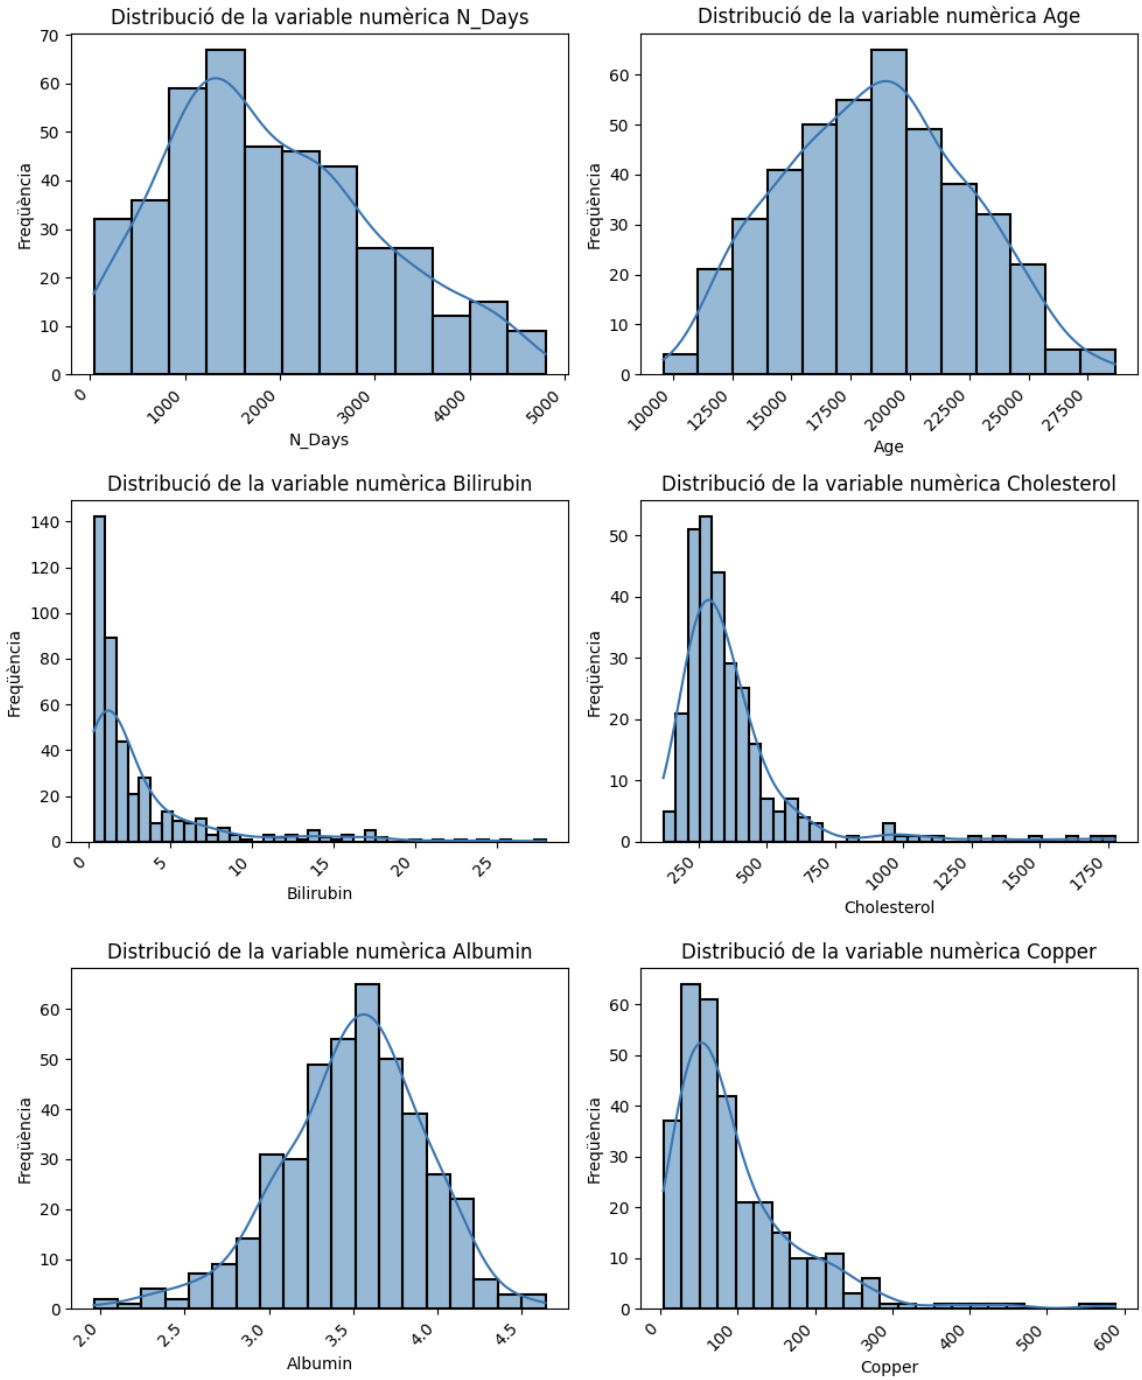
\includegraphics[width=\linewidth]{img/num-histograms-1.png}
    \caption{Histogrames de variables numèriques del datset.}
    \label{fig:num-histograms-1}
\end{figure}
\begin{figure}[H]
    \centering
    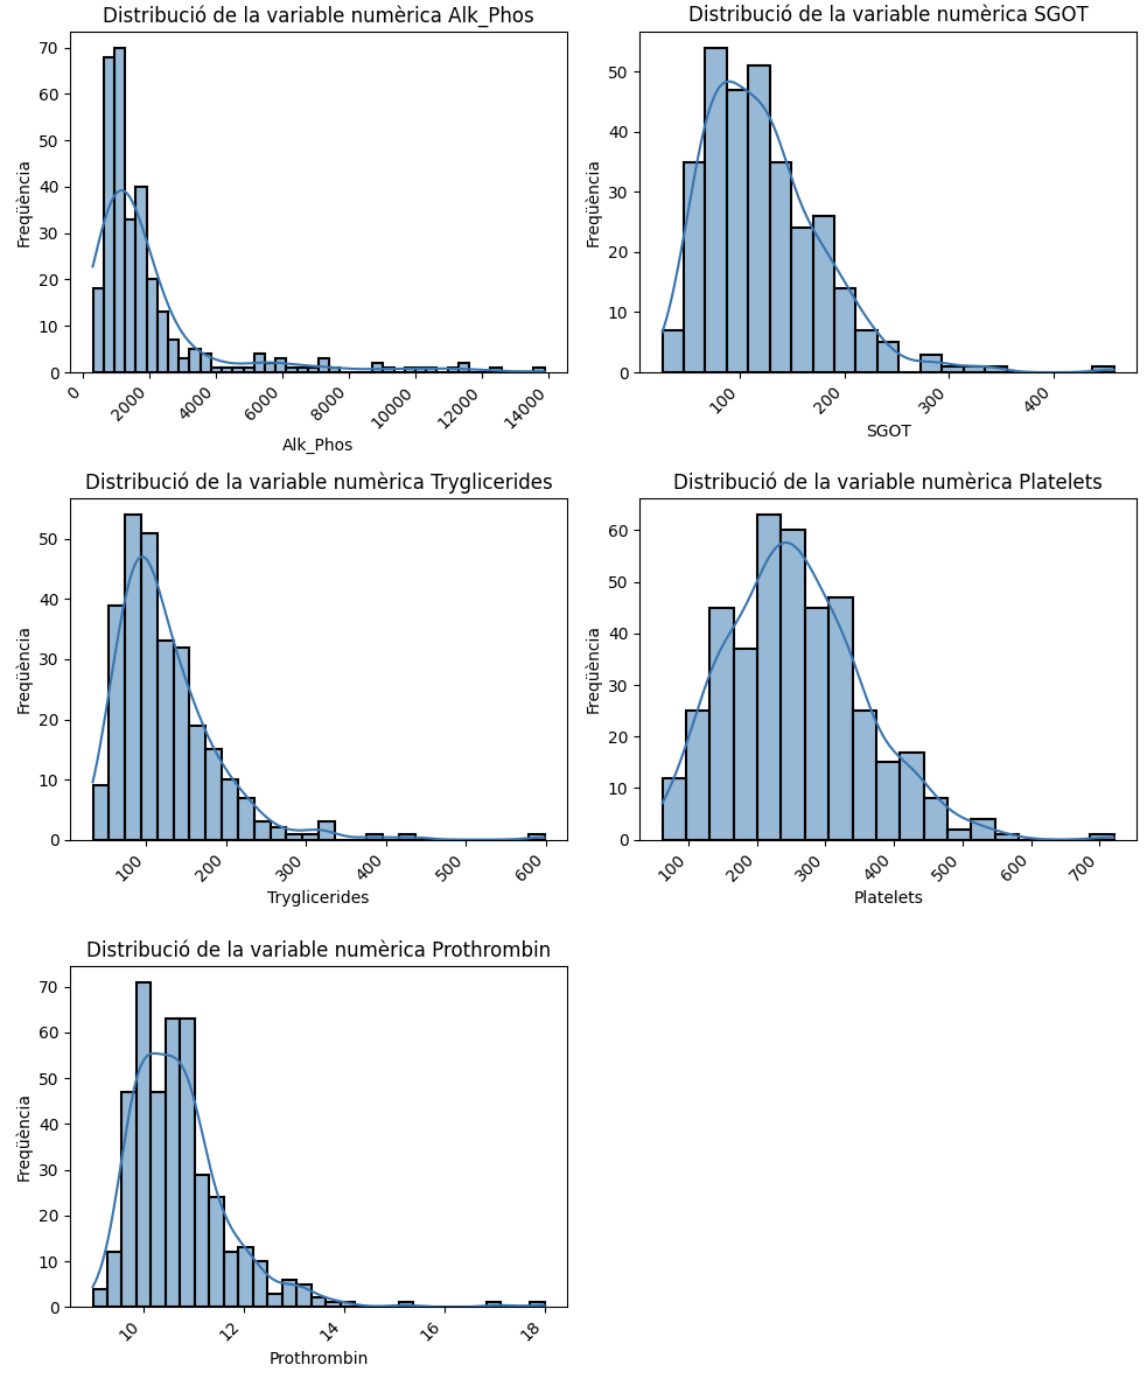
\includegraphics[width=\linewidth]{img/num-histograms-2.png}
    \caption{Histogrames de variables numèriques del datset.}
    \label{fig:num-histograms-2}
\end{figure}

En els histogrames de les diferents variables numèriques es pot veure com rarament segueixen una distribució normal. Això, en certs casos s'ha de tenir en compte en els models per tal de millorar el seu rendiment.

Per altra banda, també es pot veure que hi ha certes variables que tenen valors bastant allunyats de la distribució principal de les dades de la variable (valors atípics o outliers, que es tractaran més endavant).

\subsubsection{Variables categòriques}
En la taula \ref{tab:cat-stats-1} podem veure altres estadístiques per les variables categòriques del dataset (obtingudes mitjançant la mateixa comanda, però amb el paràmetre \texttt{include=`category'}).

\begin{table}[H]
\centering
\begin{tabular}{lrrrrrrrr}
\hline
\textbf{Statistic} & \textbf{Status} & \textbf{Drug} & \textbf{Sex} & \textbf{Ascites} & \textbf{Hepatomegaly} & \textbf{Spiders} & \textbf{Edema} & \textbf{Stage} \\ 
\hline
count & 418 & 312 & 418 & 312 & 312 & 312 & 418 & 412.0 \\ 
unique & 3 & 2 & 2 & 2 & 2 & 2 & 3 & 4.0 \\ 
top & Alive & 1 & F & 0 & 1 & 0 & NoEdema & 3.0 \\ 
freq & 232 & 158 & 374 & 288 & 160 & 222 & 354 & 155.0 \\ 
\hline
\end{tabular}
\caption{Categorical data summary of the study.}
\label{tab:cat-stats-1}
\end{table}

A més, en les figures \ref{fig:cat-countplots-1} i \ref{fig:cat-countplots-2} es poden veure els countplots de cada una de les variables categòriques, on es veu la quantitat de mostres que hi ha per cada classe de la variable, evitant els valors faltants (missings).

\begin{figure}[H]
    \centering
    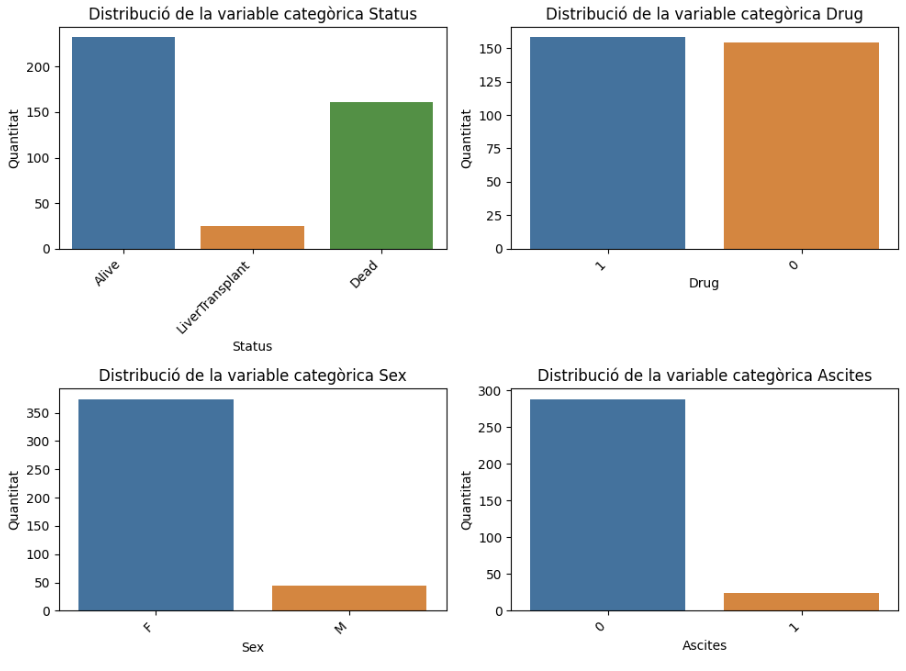
\includegraphics[width=\linewidth]{img/cat-countplots-1.png}
    \caption{Countplots de variables categòriques del datset.}
    \label{fig:cat-countplots-1}
\end{figure}
\begin{figure}[H]
    \centering
    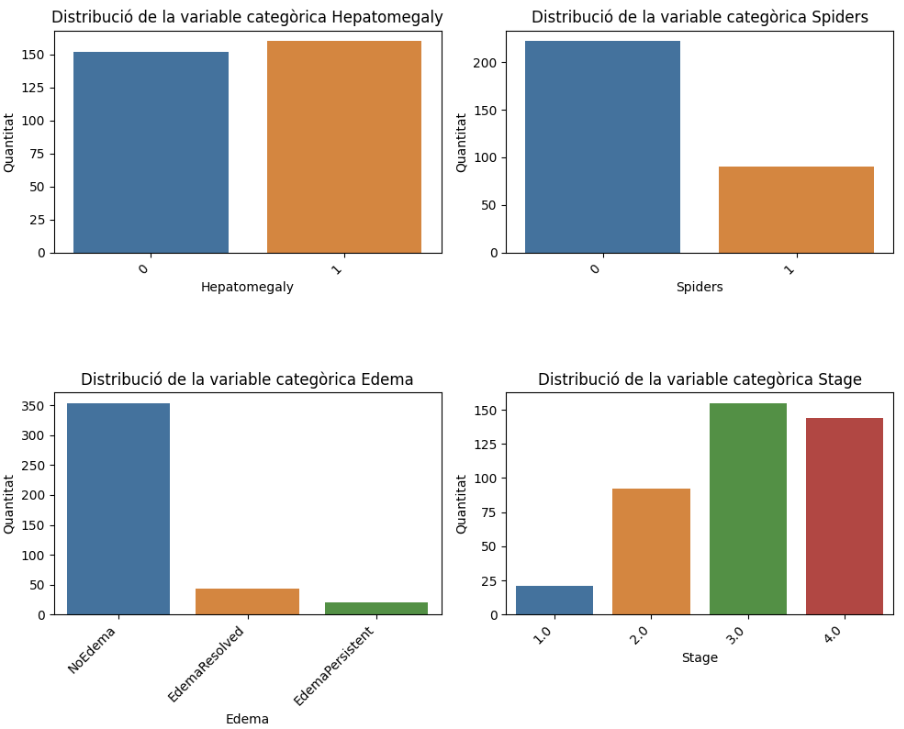
\includegraphics[width=\linewidth]{img/cat-countplots-2.png}
    \caption{Countplots de variables categòriques del datset.}
    \label{fig:cat-countplots-2}
\end{figure}

Es pot veure que les variables \textit{Status} (la variable que determinarem com a \textit{target} més endavant), \textit{Sex}, \textit{Ascites}, \textit{Spiders}, \textit{Edema} i \textit{Stage} pateixen un clar desbalanceig de classes. Per la variable \textit{Status} es contemplarà l'opció de realitzar un balanceig més endavant.

\subsection{Outliers}
El tractament d'outliers en models de Machine Learning pot ser molt important per millorar el seu rendiment mitjançant l'eliminació de mostres que es consideren atípiques. En la nostra base de dades, tal i com s'ha pogut veure en els histogrames de les variables numèriques (figures \ref{fig:num-histograms-1} i en les taules amb estadístiques de les variables (taules \ref{fig:num-histograms-2}) i en les taules \ref{tab:num-stats-1}, \ref{tab:num-stats-2} i \ref{tab:cat-stats-1}), hi ha unes quantes mostres que possiblement siguin outliers. Per exemple, la variable \textit{cholesterol} té un valor màxim de 1775, la qual cosa està exageradament per sobre de 240 (valor a partir del que es considera que una persona té un colesterol molt alt, segons la \textit{Fundación Española del Corazón} \cite{fundacioncorazon2023colesterol}).

Per eliminar aquests outliers, s'ha utilitzat l'Interquartile Range (IQR). Inicialment, un factor de multiplicació de 1,5 eliminava 119 files (un 28,47\% del dataset), resultant en menys de 300 files. Aquest valor semblava excessiu, així que s'ha optat per crear la funció \texttt{compare\_iqr\_factors()} per tal de visualitzar el percentatge de files eliminades per diversos factors multiplicatius del IQR (com es pot veure en la figura \ref{fig:iqr-factors}).

\begin{figure}[H]
	\centering
	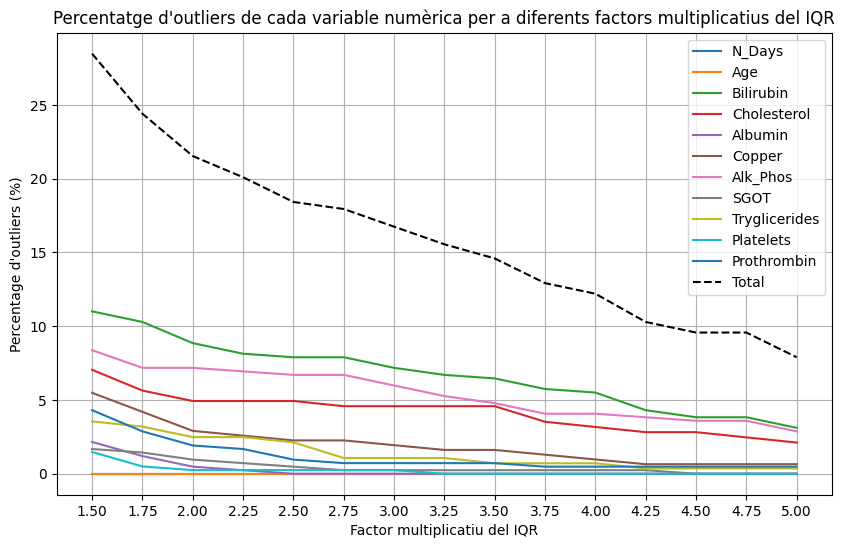
\includegraphics[width=0.85\linewidth]{img/iqr_factors}
    \caption{Percentatge de mostres considerades atípiques (outliers) en funció del factor multiplicatiu del IQR.}
    \label{fig:iqr-factors}
\end{figure}

Observant els resultats d'aquesta funció, s'ha decidit escollir un factor de 3, eliminant només 70 mostres (16,75\% del dataset). Aquesta selecció es justifica en les figures \ref{fig:outliers-1} i \ref{fig:outliers-2}, on es poden veure els histogrames i boxplots de les variables numèriques amb abans i després de l'eliminació d'outliers. En els historgrames, hi ha línia que indica a partir d'on es considera que una mostra és un outlier tenint en compte el factor de multiplicació 3. Fàcilment es pot apreciar que es consideren outliers només les mostres que se surten de la principal distribució de les dades de cada variable, reafirmant així la nostra selecció del factor de multiplicació del IQR és bona.

\begin{figure}[H]
\centering

\begin{subfigure}{.5\textwidth}
  \centering
  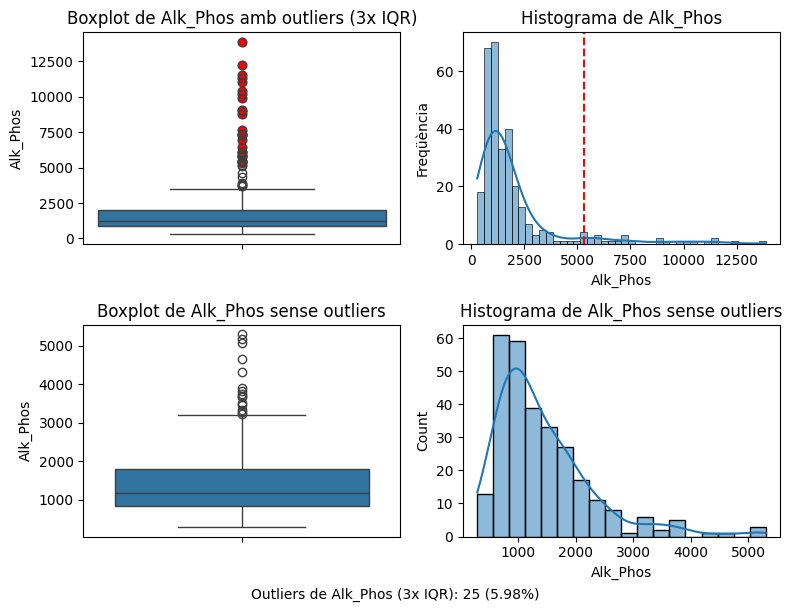
\includegraphics[width=.95\linewidth]{img/outliers_Alk_Phos.png}
  \caption{Alk\_phos}
\end{subfigure}%
\begin{subfigure}{.5\textwidth}
  \centering
  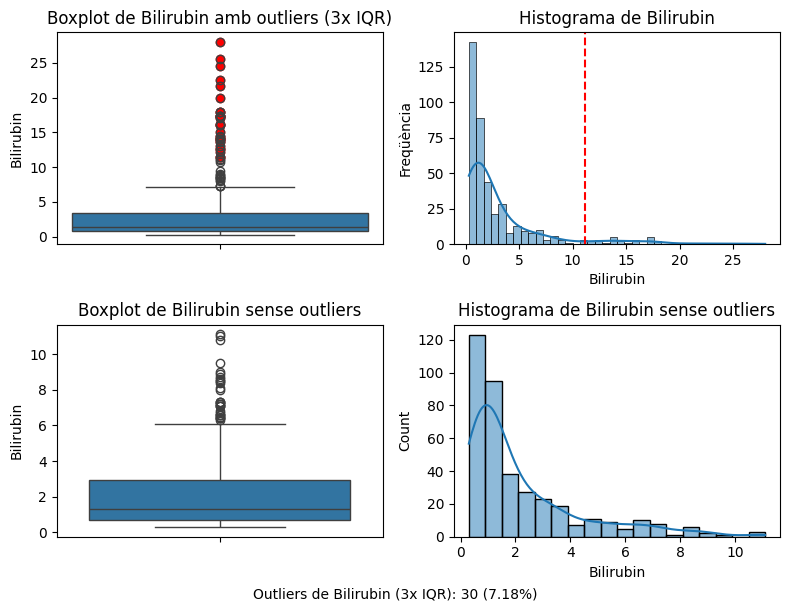
\includegraphics[width=.95\linewidth]{img/outliers_Bilirubin.png}
  \caption{Bilirubin}
\end{subfigure}
\begin{subfigure}{.5\textwidth}
  \centering
  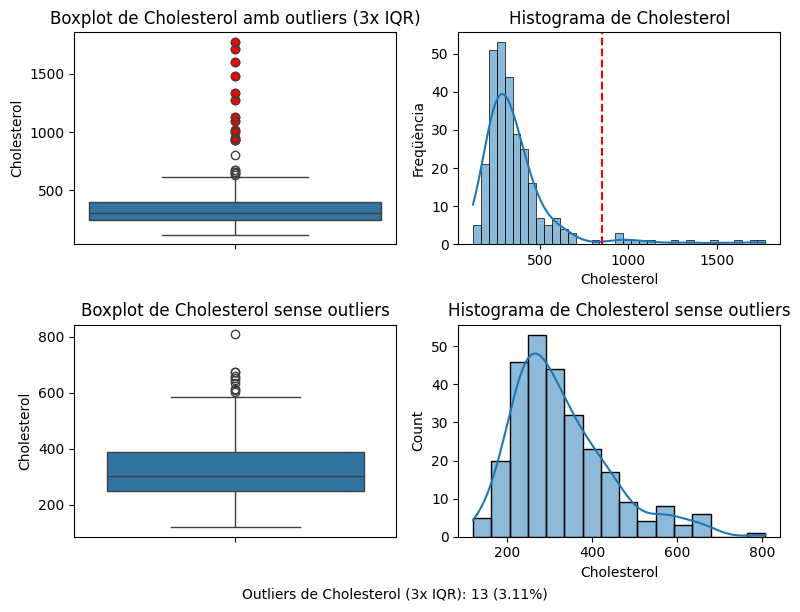
\includegraphics[width=.95\linewidth]{img/outliers_Cholesterol.png}
  \caption{Cholesterol}
\end{subfigure}%
\begin{subfigure}{.5\textwidth}
  \centering
  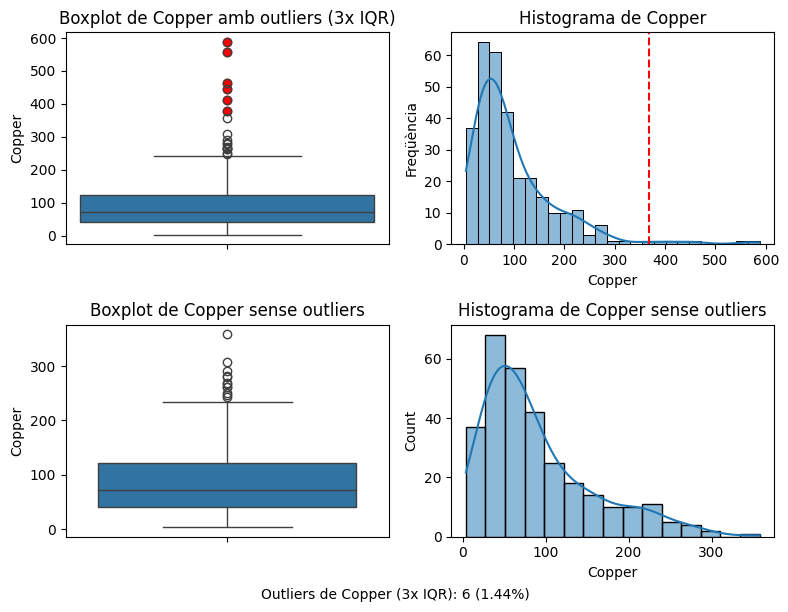
\includegraphics[width=.95\linewidth]{img/outliers_Copper.png}
  \caption{Copper}
\end{subfigure}

\caption{Distribució de dades de cada variable abans i després d'eliminar els outliers. La línia vermella discontínua dels histogramas indica a partir de on es consideren outliers les mostres. Els punts vermells dels boxplots representen outliers.}
\label{fig:outliers-1}
\end{figure}

\begin{figure}[H]
\centering

\begin{subfigure}{.5\textwidth}
  \centering
  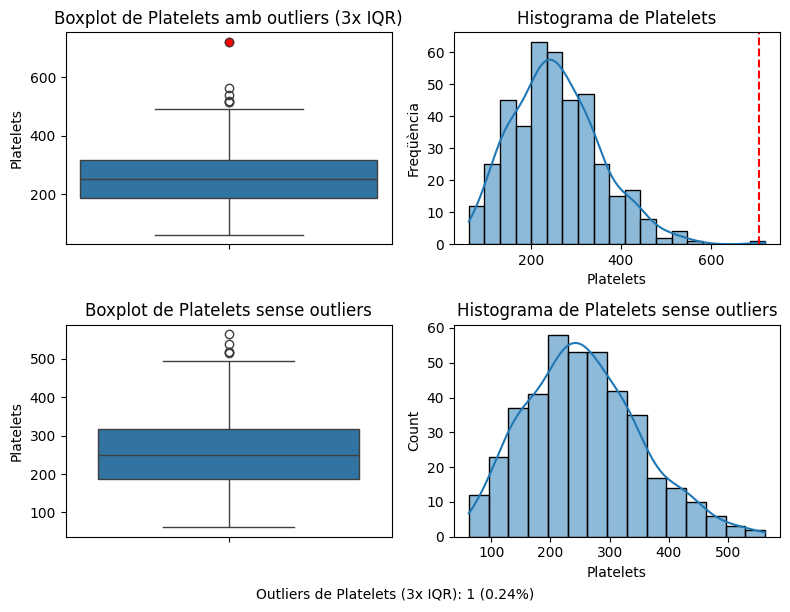
\includegraphics[width=.95\linewidth]{img/outliers_Platelets.png}
  \caption{Platelets}
\end{subfigure}%
\begin{subfigure}{.5\textwidth}
  \centering
  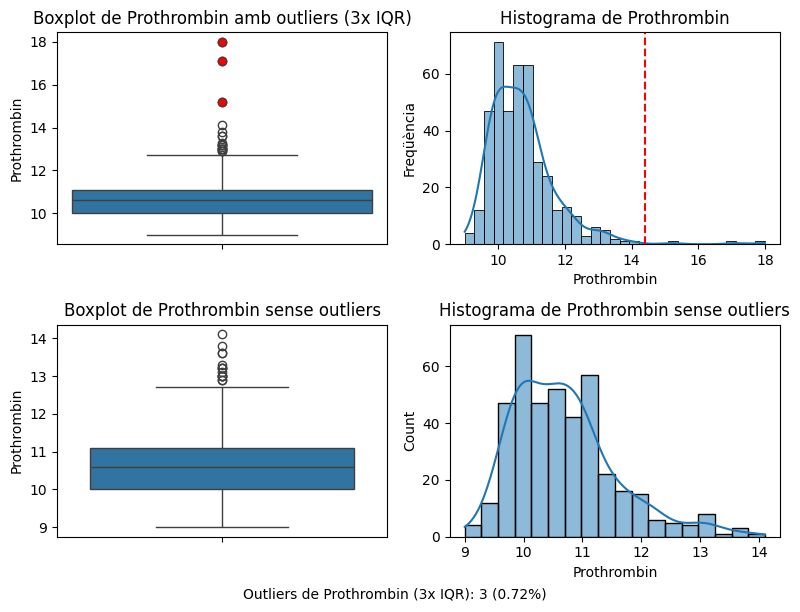
\includegraphics[width=.95\linewidth]{img/outliers_Prothrombin.png}
  \caption{Phtothrombin}
\end{subfigure}
\begin{subfigure}{.5\textwidth}
  \centering
  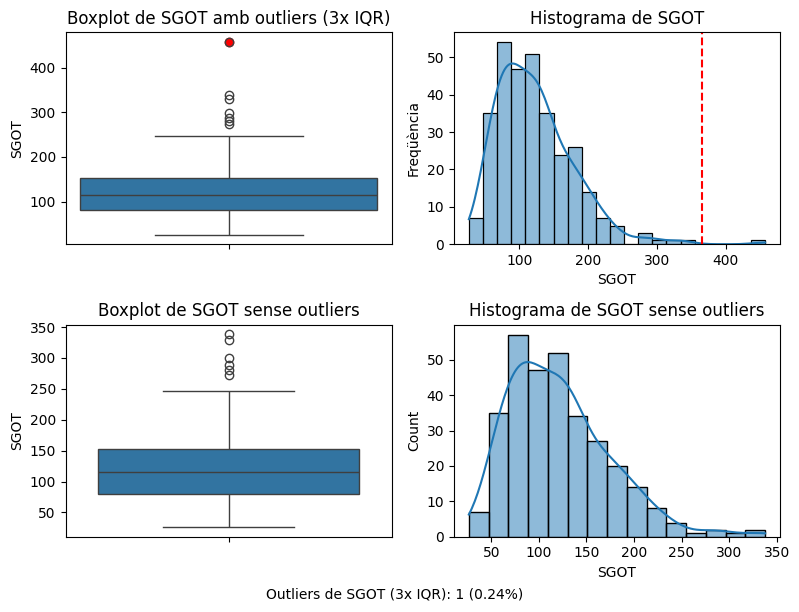
\includegraphics[width=.95\linewidth]{img/outliers_SGOT.png}
  \caption{SGOT}
\end{subfigure}%
\begin{subfigure}{.5\textwidth}
  \centering
  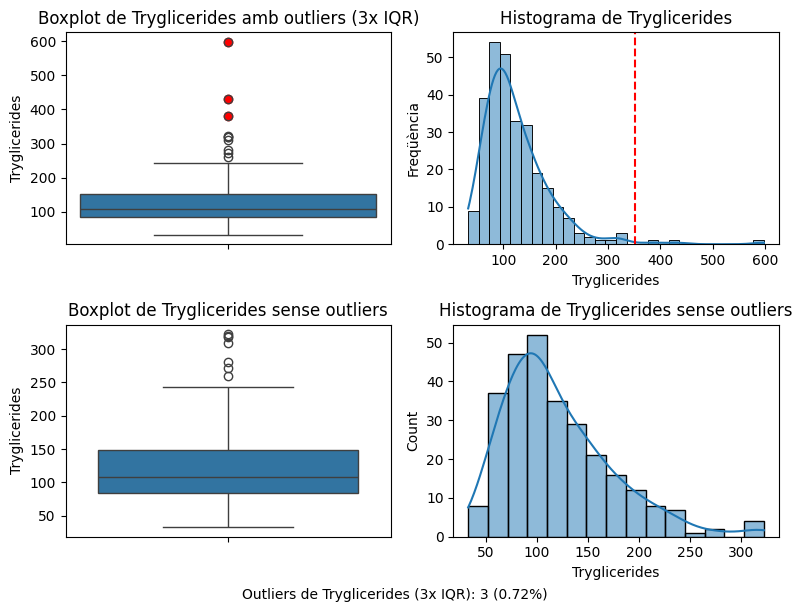
\includegraphics[width=.95\linewidth]{img/outliers_Tryglicerides.png}
  \caption{Tryglicerides}
\end{subfigure}

\caption{Distribució de dades de cada variable abans i després d'eliminar els outliers. La línia vermella discontínua dels histogramas indica a partir de on es consideren outliers les mostres. Els punts vermells dels boxplots representen outliers.}
\label{fig:outliers-2}
\end{figure}

Hem de considerar que no sempre s'obté un benefici en rendiment dels models quan s'eliminen outliers. A més, al tractar-se d'un datset amb dades de pacients malalts, podria ser que els valors que es detecten com a atípics siguin realment importants perquè el model aprengui els patrons de les dades per poder predir la nostra variable objectiu \textit{Status}. És a dir, segurament, totes les mostres del datset que contenen un nivell de colesterol extremadament alt tenen més probabilitat de morir, i eliminant outliers podem perdre part d'aquesta informació en certs casos. Per tant, l'eliminació d'outliers es valorarà per cada model més endavant, però sempre que es faci s'utilitzaran els criteris establerts en aquest estudi inicial de valors atípics (és a dir, s'utilitzarà el factor multiplicatiu del IQR de 3 mitjançant la funció \texttt{delete\_outliers}).

Per altra banda, cal mencionar que també existeix la possibilitat d'establir els valors atípics com a missings i imputar-los posteriorment. No obstant, com ja es mencionarà més endavant, ja hi ha una gran quantitat de valors faltants (missings) en el dataset, de manera que introduir-ne més només faria que hi hagués una proporció excessiva de valors imputats (que, evidentment, tenen una qualitat inferior als valors reals proporcionats en la pròpia base de dades).

\subsection{Particionat del dataset}
Per tal de poder entrenar i avaluar posteriorment els models, s'ha fet una partició del dataset en train i test. Degut a que disposem de poques mostres en la base de dades, s'ha optat per fer una partició de test de només el 15% de les dades. A més, en la partició de train es realitzarà cross validation en tots els models i també en la imputació de valors faltants per tal d'aprofitar millor la poca quantiat de mostres del datset i garantir un millor entrenament dels models.

Aquesta partició de la base de dades es fa en la funció \texttt{split\_dataset} i cal mencionar que la partició de test no s'utilitzarà en cap moment per entrenar models, ni per calcular mitjanes de cap variable del train, etc. És a dir, en tot moment es respectarà la independència de tots dos conjunts.

Finalment, cal mencionar també que, per tenir una proporció igual de classes de la variable objectiu (\textit{Status}) en tots dos conjunts, s'ha fet el perticionat mitjançant \textit{stratify} (conserva la distribució de classes en tots dos conjunts).

\subsection{Missings}
\label{subsec:missings}
Inicialment el dataset conté una gran quantitat de missings. En la taula \ref{tab:missings} es pot veure que hi ha un total de 12 variables que contenen valors faltants. Observant el dataset inicial proporcionat, es pot veure que des de l'individu amb \textit{ID} = 313 fins al final del dataset (l'últim individu té \textit{ID} = 418) hi ha múltiples columnes que no tenen ni un únic valor (concretament, 9 columnes).

\begin{table}[H]
\centering
\begin{tabular}{lr}
\hline
\textbf{Variable} & \textbf{Nº de missings} \\
\hline
Tryglicerides & 136 \\
Cholesterol & 134 \\
Copper & 108 \\
Drug & 106 \\
Ascites & 106 \\
Hepatomegaly & 106 \\
Spiders & 106 \\
SGOT & 106 \\
Alk\_phos & 106 \\
Platelets & 11 \\
Stage & 6 \\
Prothrombin & 2 \\
\hline
\end{tabular}
\caption{Quantitat de valors faltants per cada variable amb almenys 1 missing.}
\label{tab:missings}
\end{table}

El dataset té molt poques mostres (418, com hem mencionat) i això pot portar problemes a l'hora de que el model aprengui (mitjançant l'entrenament). Sabent això, s'ha decidit que l'opció d'eliminar totes les files que continguin valors faltants no és viable, ja que es reduiria dràsticament la quantitat de mostres de la base de dades i no n'hi hauria suficients per tal de que els models trobessin bons patrons en la partició de train que farem més endavant. No obstant, per aquestes files concretes en què hi ha fins a 9 columnes amb valors faltants, s'ha implementat la funció \texttt{delete\_last\_rows()}, que les elimina del datset. Més endavant es faran proves per determinar si és útil eliminar aquestes files o és millor simplement imputar els valors.

Per imputar la resta de valors faltants s'han implementat les funcions \texttt{find\_best\_imputer()} i \texttt{impute\_data()}. La funció \texttt{impute\_data()} s'encarrega d'imputar els valors amb mètodes diferents (especificats en els paràmetres que introdueix l'usuari) per les variables numèriques i per les categòriques. Si es crida a la funció amb el paràmetre \texttt{numerical\_imputer = `best'}, es cridarà internament a la funció \texttt{find\_best\_imputer()} per trobar el millor imputador numèric. Per les variables categòriques succeeix el mateix, però amb el paràmetre \texttt{categorical\_imputer = `best'}.

Per altra banda, la funció \texttt{find\_best\_imputer()} implementa cross validation (sempre amb 5 particions/\textit{folds}) per trobar el millor imputador, tant numèric com categòric. El paràmetre \texttt{X\_train} és obligatori perquè, encara que s'estiguin intentant imputar els valors de la partició de test (que es menciona més endavant), s'escullen els millors mètodes d'imputació mitjançant només valors del train, per respectar totalment la independència entre les particions d'entrenament i de prova. El cross validation es fa sobre les mostres del train que no contenen missings i consisteix en generar artificialment valors faltants en cada \textit{fold} per posteriorment imputar-los i comprovar la seva eficàcia. Els mètodes d'imputació que es proven són els següents:
\begin{itemize}
	\item \textbf{Variables numèriques:}
		\begin{itemize}
		\item \textbf{KNNImputer:} aquest imputador es prova amb diferents valors de l'hiperparàmetre \textit{k} (1, 2, 3, 5, 10, 15, 20, 25, 50) i pot ser molt útil degut a que intenta imputar els valors basant-se en la mitjana dels valors dels deus \textit{k} veïns més propers.
		
		\item \textbf{SimpleImputer (mitjana):} aquest imputador és molt senzill. Simplement substitueix els valors faltants per la mitjana de la variable en què es trobi el valor missing. Generalment aquest mètode és pitjor que la resta, però s'ha volgut incloure igualment per si en algun cas proporciona un millor rendiment.
		
		\item \textbf{IterativeImputer (Linear Regression):} aquesta tècnica d'imputació és més complexa que les anteriors. L'iterative imputer pretén imputar els valors de cada variable mitjançant combinacions lineals de les altres. En aquest cas, es crea un model de regressió lineal per cada variable amb les altres variables com a predictores (sense tenir en compte els valors missing) i es fa una predicció per cada valor faltant. Al estar utilitzant una regressió lineal, el model rendirà millor si hi ha més relacions lineals entre variables numèriques del dataset.
		\end{itemize}

	\item \textbf{Variables categòriques:}
	Per les variables categòriques s'ha decidit utilitzar només classificadors, ja que altres mètodes no sempre funcionen per variables categòriques. S'ha de tenir en compte que en el moment d'imputar les dades encara no s'ha codificat el dataset (ja que codificar un dataset amb calors faltants és relativament complex i sovint genera errors). Per tant, les variables categòriques no poden ser utilitzades per algoritmes com ara KNN per tal de calcular les distàncies entre mostres. Per tant, predicció (imputació) de variables categòriques es fa, per cada variable categòrica, entrenant el classificador amb les variables numèriques.
	\begin{itemize}
		\item \textbf{KNeighborsClassifier:} aquest classificador obté resultats bastant diferents en funció de l'hiperparàmetre \textit{k}. Em aquest cas, es proven els mateixos valors de \textit{k} que en el KNNImputer utilitzat en les variables numèriques. Aquest classificador basa les seves prediccions en la moda (valor més freqüent) dels seus \textit{k} veïns més propers.
		\item \textbf{DecisionTreeClassifier:} en aquest cas s'imputen els valors mitjançant prediccions d'un arbre de decisió. Aquest arbre de decisió realitzarà, per cada variable categòrica, diverses particions del dataset en conjunts intentant mantenir homogeneïtat en cada un d'ells i posteriorment imputarà el valor faltant mitjançant la classe més freqüent en el conjunt on es situï la mostra a predir. En el nostre cas provem dos models, un amb el criteri d'entropia (entropy) i l'altre amb gini.
		
		\item \textbf{RandomForestClassifier:} aquest classificador es crea múltiples arbres de decisió i combina les seves prediccions. Generalment, el rendiment d'aquest classificador és més alt que el d'un sol arbre de decisió. En el nostre cas, també es prova tant amb el criteri entropy com amb gini.
	\end{itemize}
\end{itemize}

Tant els models de Decision Tree com els de Random Forest tenen bastants paràmetres que modifiquen el seu rendiment, especialment controlant si l'arbre fa més o menys overfitting. No obstant, s'ha decidit deixar els paràmetres per defecte per tal de no tenir una quantitat excessiva de models a provar en la funció \texttt{find\_best\_imputer()} i així reduir el cost computacional (i temps d'execució) d'aquesta funció. Més endavant, en el propi model de predicció de la variable objectiu mitjançant l'arbre de decisió, sí que es provaran diferents combinacions de paràmetres.

Pel que fa a l'elecció del millor model d'imputació, s'ha decidit que per les variables numèriques s'utilitzarà la mètrica de $R^2$ (coeficient de determinació). Un valor alt d'aquest coeficient significa que el model de imputació ha capturat un gran part de la variància dels valors reals, indicant que els valors predits s'assimilen als reals. S'ha escollit aquesta mètrica degut a que no depèn de l'escala de les dades, és robusta a outliers i és fàcilment interpretable.

Per altra banda, per avaluar l'imputador categòric s'ha decidit utilitzar la mètrica de \textit{f1}, ja que considera tant la precisió com el recall. A més, utilitzem la versió \textit{weighted} (ponderada) de la mètrica \textit{f1} per tal de tenir en compte el desbalanceig de les classes i per garantir que no s'obté una millor puntuació simplement pel fet d'estar predint (imputant) la classe majoritària de la variable.

En general, com es mencionarà més endavant, tots els models predictors de la variable target (\textit{Status}) també faran servir la mètrica de \textit{f1-score-weighted} pels mateixos motius.

Finalment, cal mencionar que la imputació de valors faltants sempre es farà per separat en les particions de train i test, per evitar data leakage i mantenir la independència dels dos conjunts.

\subsection{Recodificació de variables}
Com ja hem mencionat, en els models d'imputació de dades no s'han pogut tenir gaire en compte les variables categòriques degut a que no es poden fer operacions si no estan representades com a valors numèrics. Per altra banda, en el preprocessament inicial ja s'han passat certs valors de variables categòriques a format numèric per tal de poder treballar-hi més fàcilment. No obstant, ara que ja no hi ha valors faltants en el datset, pot ser molt útil realitzar una codificació de les variabels categòriques perquè els models de predicció de la variable objectiu (\textit{Status}) les puguin tenir en compte.

Hi ha múltiples mètodes de codificació de variables categòriques, com ara One Hot Encoding, Label Encoding, Ordinal Encoding, etc. Inicialment es va plantejar l'us de One Hot Encoding, però aquest codificador augmenta molt la dimensionalitat del dataset, redueix l'eficàcia dels càlculs, no manté la naturalesa dels valors de certes variables i dificulta molt la interpretació de la base de dades (crucial a l'hora de generar gràfics, comprovar que no hi hagi errors de valors en el dataset, etc.). Amb tot això, s'ha decidit descartar aquest encoder.

Pel que fa al Label Encoding i Ordinal Encoding, tots dos són bastant similars en el sentit de que simplement etiqueten cada una de les classes de les variables categòriques amb un número. No obstant, s'ha decidit utilitzar Ordinal Encoding, ja que hi ha variables que tenen un ordre natural en elles (com ara els valors de \textit{Stage}, que segueixen un ordre en funció de la fase en la que es trobi el pacient. És a dir, la fase 1 i la 3 estan ``més lluny'' que la 3 i la 4). Hi ha altres variables que no tenen un ordre en concret, però la majoria d'aquestes són binàries i no es veuran gaire afectades negativament pel fet de fer Ordinal Encoding. De fet, certs models com ara els arbres de decisió es poden veure beneficiats pel fet de tenir variables binàries (o que no tenen un ordre natural) expressades mitjançant Ordinal Encoding.

La codificació de variables es fa en la funció \texttt{encode\_variables}. Més endavant es faran proves per veure si és necessari fer encoding en tots els models o només en alguns.
